
%%% Local Variables:
%%% mode: latex
%%% TeX-master: t
%%% End:

\documentclass[xcolor=svgnames,11pt]{beamer}
\usepackage[utf8]{inputenc}
\usepackage[english]{babel}
\usepackage{hyperref}
\usepackage{mathrsfs}
\usepackage{geometry}
\usepackage{listings}
\usepackage{graphicx}
\usepackage{xspace}
\usepackage{verbatim}
\usepackage{textcomp}
\usepackage{amsmath}
\usepackage{amsfonts}
\usepackage{syntax}
\usepackage{amssymb}
\usepackage{mathtools}
\usepackage{subcaption}
\usepackage{textgreek}
\usetheme{Frankfurt}
\usecolortheme{crane}

\usepackage{../mathpartir}

\beamertemplatenavigationsymbolsempty
\usepackage{tikz}
\usetikzlibrary{backgrounds,positioning,shapes,
  shadings,shadows,arrows,decorations.markings,calc,fit,fadings}
\input{../tikz}

\newcommand{\mysc}[1]{\textsc{#1}\xspace}
\newcommand{\coq}{\textsc{Coq}\xspace}
\newcommand{\agda}{\textsc{Agda}\xspace}
\newcommand{\ma}{\textsc{microAgda}\xspace}
\newcommand{\na}{\textsc{nanoAgda}\xspace}

\lstset{
  tabsize=4,
  aboveskip={0.4\baselineskip},
  belowcaptionskip=0.4\baselineskip,
  columns=fixed,
  showstringspaces=false,
  extendedchars=true,
  breaklines=true,
  frame=none,
  xleftmargin=\parindent,
  basicstyle=\footnotesize\ttfamily,
  keywordstyle=\bfseries\color{green!30!black},
  keywordstyle=[2]\bfseries\color{red!50!white},
  commentstyle=\itshape\color{purple!40!black},
  identifierstyle=\color{blue!30!black},
  stringstyle=\color{orange},
}

\lstdefinelanguage{Agda}{
  morekeywords={data,where,case,let,in},
  literate={->}{{$\to{}$}}1 {xx}{{$\times$}}1 {==}{{$\equiv$}}1 {*}{{$\times$}}1,
}

\lstdefinelanguage{nanoAgda}{
  morekeywords={case,of,split,rec},
  literate={->}{{$\to$}}1 {\\}{{$\lambda$}}1 {'}{`}1
    {*}{{$\times$}}1 {*0}{{$\star_0$}}2 {*1}{{$\star_1$}}2 {*2}{{$\star_2$}}2,
}
\lstset{
  aboveskip=0pt,
  belowcaptionskip=0pt,
  basicstyle=\small\ttfamily,
  escapeinside={!}{!},
}


\addtobeamertemplate{footline}{
\hfill
\insertframenumber/20 \hspace{1mm}
\vspace{2 mm}
}

\title{A sequent-calculus presentation of type-theory}
\author[Gabriel Radanne]{Gabriel Radanne\\ Under the supervision of Jean-Philippe Bernardy}
\institute[ENS Rennes]{ENS Rennes --- Chalmers University of Technology}

\begin{document}

\begin{frame}[plain]
\titlepage
\end{frame}

\begin{frame}{Plan}
\tableofcontents%[section]
\end{frame}

\section{An Introduction to dependent types}

\begin{frame}[fragile]
  Imagine we want to define lists, but with guarantees on the length of the list.

  We have the length operation:

\alt<1>{$|$ \lstinline[language=caml,basicstyle=\ttfamily]{['a' ; 'b' ; 'c']} $| = 3$.}{$|$ \lstinline[language=caml,basicstyle=\ttfamily]{ 'a' :: 'b' :: 'c' :: []} $| = 3$.}

  \pause\pause
  \ \\We can define the head function like this in \mysc{OCaml}:
\begin{lstlisting}[language=caml]
let head x = match x with
  | [] -> failwith "PANIC" !\only<4->{\\\color{Gray}We want the type-system to ensure this doesn't happen.}!
  | (h::t) -> h
\end{lstlisting}\pause

\lstinline[language=caml,basicstyle=\ttfamily]{head l}
should only be valid if $|$\lstinline[language=caml,basicstyle=\ttfamily]{l}$|>0$.
\end{frame}

\begin{frame}[fragile]
  Let's start by natural numbers:
\begin{lstlisting}[language=Agda]
data Nat : Set where
Zero : Nat
Succ : Nat -> Nat
\end{lstlisting}\pause

\begin{lstlisting}[language=Agda]
three : Nat
three = Succ (Succ (Succ Zero))
\end{lstlisting}\pause

  We can now define a special kind of list:
\begin{lstlisting}[language=Agda]
data Vec (A : Set) : Nat -> Set where
Nil : Vec A Zero
Cons : {n : Nat} -> A -> Vec A n -> Vec A (Succ n)
\end{lstlisting}\pause

\begin{lstlisting}[language=Agda]
myVec : Vec Char three
myVec = Cons 'a' (Cons 'b' (Cons 'c' Nil))
\end{lstlisting}

\end{frame}

\begin{frame}[fragile]
\begin{lstlisting}[basicstyle=\footnotesize\ttfamily,language=Agda]
data Nat : Set where
Zero : Nat
Succ : Nat -> Nat
\end{lstlisting}
\begin{lstlisting}[basicstyle=\footnotesize\ttfamily,language=Agda]
data Vec (A : Set) : Nat -> Set where
Nil : Vec A Zero
Cons : {n : Nat} -> A -> Vec A n -> Vec A (Succ n)
\end{lstlisting}

\ \\The head function:
\begin{lstlisting}[language=Agda]
head : forall { A n } -> Vec A (Succ n) -> A
head (Cons x xs) = x
\end{lstlisting}\pause

\ \\
\begin{lstlisting}[language=Agda]
  head Nil !\color{Gray}$\gets$ This is a type error.!
\end{lstlisting}
\end{frame}

\begin{frame}[fragile]
\begin{lstlisting}[basicstyle=\footnotesize\ttfamily,language=Agda]
data Nat : Set where
Zero : Nat
Succ : Nat -> Nat
\end{lstlisting}
\begin{lstlisting}[basicstyle=\footnotesize\ttfamily,language=Agda]
data Vec (A : Set) : Nat -> Set where
Nil : Vec A Zero
Cons : {n : Nat} -> A -> Vec A n -> Vec A (Succ n)
\end{lstlisting}

\ \\When we concatenate two vectors, $|$\lstinline[language=caml,basicstyle=\ttfamily]{append l l'}$| = |$
\lstinline[language=caml,basicstyle=\ttfamily]{l}$| + |$
\lstinline[language=caml,basicstyle=\ttfamily]{l'}$|$.\pause
\begin{lstlisting}[language=Agda]
append : forall { n m A } ->
    Vec A n -> Vec A m -> Vec A (n + m)
append Nil ys = ys
append (Cons x xs) ys = Cons x (append xs ys)
\end{lstlisting}
\end{frame}

\begin{frame}{Dependent types}
What have we done?
\begin{itemize}
\item We defined a type with a {\bf term} as parameter:
\lstinline[language=Agda,basicstyle=\ttfamily]{Vec A n}.\pause
\item We used these values to enforce properties.\pause.. by type-checking.\pause
\item We manipulated these values inside the type: \lstinline[language=Agda,basicstyle=\ttfamily]{Vec A (n+m)}.
\end{itemize}\pause

Types depends on terms.
\end{frame}

\begin{frame}{Dependent types}
\begin{columns}
\column{0.6\textwidth}
Dependent types:
\begin{itemize}
\item<2-> Strongly related to Curry-Howard Isomorphism.
\item<3-> Introduce as a type-theory by Martin-Löf in 1971. Proposed as foundation of mathematics.
\item<4-> Has gained popularity recently for theorem-proving with \coq,
\item<5-> but also in programming: {\only<6>{\bf}\agda}, \mysc{Idris}, \mysc{ATS},\dots
\end{itemize}
\column{0.4\textwidth}
\uncover<3->{
\begin{figure}[htbp]
  \centering
  \includegraphics[width=\linewidth]{../martin-lof}

  Martin-Löf
\end{figure}
}
\end{columns}
\end{frame}

\section{Limitations of current typecheckers}
\begin{frame}
  \frametitle{Limitations of current typecheckers}
  \tableofcontents[currentsection]
\end{frame}

\subsection{Efficiency issues}
\begin{frame}{Efficiency issues}
  \agda's type checker uses a natural deduction style:
  \begin{itemize}
  \item Inference duplicates parts of terms.
  \item These parts are not shared in the \agda core representation anymore.
  \item Typechecking must be done multiple times, causing performance penalties.
  \end{itemize}
  \begin{figure}
    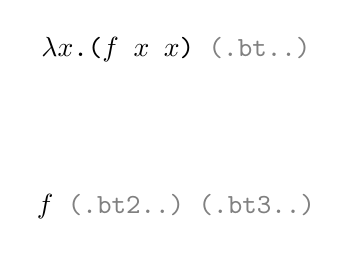
\begin{tikzpicture}
      \node[anchor=center] (lambda) at (0,0) {
        \texttt{$\lambda{}x$.($f$ $x$ $x$) {\color{Gray}(.\tikzcoord{bt}..)}}
      };
      \node[anchor=center, text centered] (lambda2) at (0,-2) {
        \texttt{$f$\ {\color{Gray}(.\tikzcoord{bt2}..)\ (.\tikzcoord{bt3}..)}}
      };
    \end{tikzpicture}
    \centering
  \end{figure}
  \begin{tikzpicture}[remember picture, overlay]
    \node[xshift=0.1cm,yshift=-0.2cm, coordinate] (bt') at (bt) {} ;
    \draw[remember picture, -latex] (bt') to[out=-90,in=90] ($(bt2)+(0.1,0.3)$) ;
    \draw[remember picture, -latex] (bt') to[out=-90,in=90] ($(bt3)+(0.1,0.3)$) ;
  \end{tikzpicture}
\end{frame}

\subsection{The ``case decomposition'' issue}
\begin{frame}{The ``case decomposition'' issue}
  Natural deduction style makes propagating typing constraints to subterms difficult.

  For example, \agda's typechecker has no knowledge of which branch was taken while it typechecks the body of a case.
  \begin{center}
    \begin{minipage}{0.9\textwidth}
      \lstinputlisting[basicstyle=\ttfamily,language=Agda]{../poster/case.agda}
    \end{minipage}
  \end{center}
\end{frame}

\subsection{The monolithic approach}
\begin{frame}{The monolithic approach}
  \agda currently does not have a core language that can be reasoned about and formally verified.

  \coq, on the other hand, is built as successive extensions of a core language (CIC).
  \begin{figure}[htbp]
    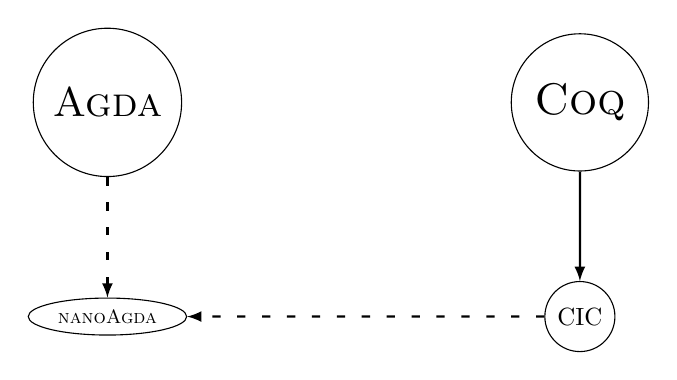
\begin{tikzpicture}[yscale=0.4, xscale=0.4]
      \node[draw, circle, scale=1.6] (Coq) at (8,3) {\coq} ;
      \node[draw, circle, scale=0.9] (CCC) at (8,-3.8) {CIC} ;
      \node[draw, circle, scale=1.5] (agda) at (-7,3) {\agda} ;
      % \node[draw, ellipse, scale=0.9] (ma) at (-7,3) {\ma} ;
      \node<2>[draw, ellipse, scale=0.7] (na) at (-7,-3.8) {\na} ;
      \draw[-latex,thick] (Coq) -- (CCC) ;
      % \draw[-latex,thick] (ma) -- (na) ;
      \draw<2>[-latex,thick, loosely dashed] (agda) to (na) ;
      \draw<2>[-latex,thick, loosely dashed] (CCC) to (na) ;
    \end{tikzpicture}
    \centering
  \end{figure}
\end{frame}

\section{\na and \ma}

\subsection{Goals}
\begin{frame}{Goals}
  Our goals are to have a language that is:
  \begin{itemize}
  \item<1-> A type-theory: Correctness should be expressible via types.
  \item<2-> Low-level: One should be able to translate high-level languages into this language while retaining properties such as run-time behaviour, complexity, etc.
  \item<3-> Minimal: The language should be well defined and it should be possible to formally verify the type-checking algorithm.
  \end{itemize}
\end{frame}

\subsection{\na}
\begin{frame}[fragile]{\na}
\begin{columns}
\column{0.5\textwidth}
\begin{lstlisting}[language=Agda]
id : !\tikzcoord{a1}!(a : Set) -> !\tikzcoord{b1}!a -> !\tikzcoord{c1}!a!\tikzcoord{a2}!
id _ x = x
\end{lstlisting}
\centering in \agda
\column{0.6\textwidth}
\pause
\begin{lstlisting}[basicstyle=\scriptsize\ttfamily,language=nanoAgda]
TERM
f = \a -> (
      f' = \x -> (r=x; r);
      f' ) ;
f
TYPE
set = *0 ;
!\tikzcoord{z1}!f_ty = (a : set) -> (
            !\tikzcoord{x1}!a' = a ;
            a2a = (x : a') -> !\tikzcoord{y1}!a';!\tikzcoord{x2}!
            a2a!\tikzcoord{x3}!
    ) ;
f_ty!\tikzcoord{z2}!
\end{lstlisting}
\centering in \na
\end{columns}
\begin{tikzpicture}[remember picture, overlay]
  \coordinate (a2') at ($(a2)+(0,1.3mm)$) {} ;
  \coordinate (x1') at ($(x1)+(0,1.3mm)$) {} ;
  \coordinate (z1') at ($(z1)+(0,1.3mm)$) {} ;
  \coordinate (x2') at ($(x2)+(0,1.3mm)$) {} ;
  \node<3>[opacity=0.4, fill=yellow, fit=(a1) (a2')] {};
  \node<3>[opacity=0.4, fill=yellow, fit=(z1') (z2) (x2)] {};
  \node<4>[opacity=0.4, fill=yellow, fit=(b1) (a2')] {};
  \node<4>[opacity=0.4, fill=yellow, fit=(x1') (x2) (x3)] {};
  \node<5>[opacity=0.4, fill=yellow, fit=(c1) (a2')] {};
  \node<5>[opacity=0.4, fill=yellow, fit=(y1) (x2')] {};
\end{tikzpicture}
\end{frame}

\begin{frame}{Sequent calculus}
  There are various definitions of sequent calculus. Here, we mean that every intermediate result or sub-term are bound to a variable.
  % \alt<2->{
    \begin{figure}
      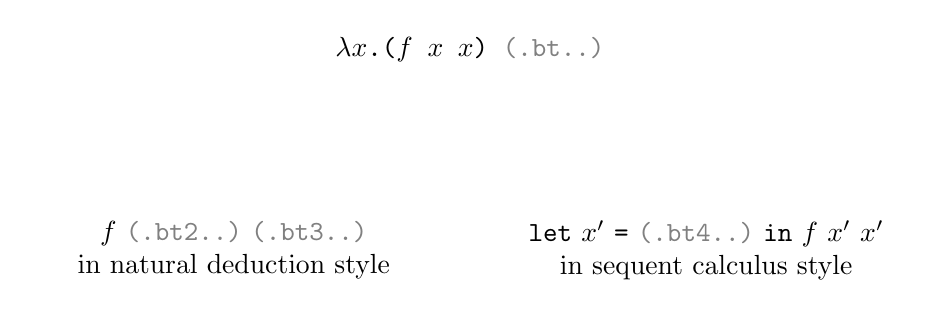
\begin{tikzpicture}[yscale=1.7]
        \node (lambda) at (0,0) {
          \texttt{$\lambda{}x$.($f$ $x$ $x$) {\color{Gray}(.\tikzcoord{bt}..)}}
        };
        \node[text centered, text width=5cm] (lambda2) at (-3,-1.5) {
          \texttt{$f$\ {\color{Gray}(.\tikzcoord{bt2}..)\ (.\tikzcoord{bt3}..)}}\\
          in natural deduction style
        };
        \uncover<2->{\node[text centered, text width=5cm] (lambda3) at (3,-1.5) {
          \texttt{let $x'$ = {\color{Gray}(.\tikzcoord{bt4}..)}\ in $f$ $x'$ $x'$}\\
          in sequent calculus style
        };}
      \end{tikzpicture}
      \centering
    \end{figure}
  \begin{tikzpicture}[remember picture, overlay]
    \node[xshift=0.1cm,yshift=-0.2cm, coordinate] (bt') at (bt) {} ;
    \draw[remember picture, -latex] (bt') to[out=-90,in=80] ($(bt2)+(0.1,0.3)$) ;
    \draw[remember picture, -latex] (bt') to[out=-90,in=60] ($(bt3)+(0.1,0.3)$) ;
    \draw<2->[remember picture, -latex] (bt') to[out=-90,in=90] ($(bt4)+(0.1,0.3)$) ;
  \end{tikzpicture}
  % }{
    % \begin{figure}[htbp]
    %   \lstinputlisting[language=Caml]{seq.ml}
    %   \centering
    % \end{figure}
  % }
\end{frame}

\begin{frame}[shrink,fragile]{Presentation of the language}
\begin{itemize}
\item \textbf{Variables}:
  \textbf{Hypotheses} $x$ and \textbf{Conclusions} $\overline{x}$
\end{itemize}
\begin{center}
  \setlength{\tabcolsep}{10pt}
  \vspace{-10pt}
  \begin{tabular}{r l l l}
    \uncover<2->{{\bf Functions} & $\lambda x. t$ & $(f\ \overline{x})$ & $(x:\overline{Y})\to T$ \\}
    \uncover<3->{{\bf Pairs} &
    $(\overline{x},\overline{y})$ & $x.1$ &\ $(x:\overline{Y})\times T$\\}
    \uncover<4->{{\bf Enumerations} & $`l$ & \texttt{case} & $\{`l_1,`l_2,\dots\}$\\}
  \end{tabular}
\vspace{-30pt}
\end{center}
\begin{itemize}
\item<5-> {\bf Constructions and Destructions}:\\
  {\tt let} $\overline{x} = c$ \ and\   {\tt let} $x = d$
\item<6-> {\bf Universes}:\\
  $\star_i$ with $i\in\mathbb{N}$ \qquad $\star_0$ is equivalent to \texttt{Set}
\item<7-> {\bf Relation between Conclusions and Hypotheses}:\\
  \texttt{let} $\overline{x}$ = $y$ {\color{Gray}A conclusion can be defined as an hypothesis.}

  \uncover<8->{\texttt{let} $x$ = $(\overline{y}:\overline{Z})$ {\color{Gray}The cut construction.}}
\end{itemize}
\end{frame}

\subsection{\ma}
\begin{frame}[fragile]{\ma}
A new syntax, easier to manipulate, and that can be translated easily into \na.\pause

\ \\
\begin{columns}
\column{0.5\textwidth}
\begin{lstlisting}[language=Agda]
id : !\tikzcoord{a1}!(a : Set) -> !\tikzcoord{b1}!a -> !\tikzcoord{c1}!a!\tikzcoord{a2}!
id _ x = x
\end{lstlisting}
\centering in \agda

\ \\
\begin{lstlisting}[language=nanoAgda]
TERM
  \a -> \x -> x

TYPE
  !\tikzcoord{e1}!(a : *1) -> !\tikzcoord{f1}!(x : a) -> !\tikzcoord{g1}!a!\tikzcoord{e2}!
\end{lstlisting}
\centering in \ma
\column{0.6\textwidth}
\pause
\begin{lstlisting}[basicstyle=\scriptsize\ttfamily,language=nanoAgda]
TERM
f = \a -> (
      f' = \x -> (r=x; r);
      f' ) ;
f
TYPE
set = *0 ;
!\tikzcoord{z1}!f_ty = (a : set) -> (
            !\tikzcoord{x1}!a' = a ;
            a2a = (x : a') -> !\tikzcoord{y1}!a';!\tikzcoord{x2}!
            a2a!\tikzcoord{x3}!
    ) ;
f_ty!\tikzcoord{z2}!
\end{lstlisting}
\centering in \na
\end{columns}
\begin{tikzpicture}[remember picture, overlay]
  \coordinate (a2') at ($(a2)+(0,1.3mm)$) {} ;
  \coordinate (e2') at ($(e2)+(0,1.3mm)$) {} ;
  \coordinate (x1') at ($(x1)+(0,1.3mm)$) {} ;
  \coordinate (z1') at ($(z1)+(0,1.3mm)$) {} ;
  \coordinate (x2') at ($(x2)+(0,1.3mm)$) {} ;
  \node<4>[opacity=0.4, fill=yellow, fit=(e1) (e2')] {};
  \node<4>[opacity=0.4, fill=yellow, fit=(a1) (a2')] {};
  \node<4>[opacity=0.4, fill=yellow, fit=(z1') (z2) (x2)] {};
  \node<5>[opacity=0.4, fill=yellow, fit=(f1) (e2')] {};
  \node<5>[opacity=0.4, fill=yellow, fit=(b1) (a2')] {};
  \node<5>[opacity=0.4, fill=yellow, fit=(x1') (x2) (x3)] {};
  \node<6>[opacity=0.4, fill=yellow, fit=(g1) (e2')] {};
  \node<6>[opacity=0.4, fill=yellow, fit=(c1) (a2')] {};
  \node<6>[opacity=0.4, fill=yellow, fit=(y1) (x2')] {};
\end{tikzpicture}
\end{frame}

\subsection{Results}
\begin{frame}{Results}
\begin{itemize}
\item We implemented a typechecker and evaluator for \na.
\item We introduced a new intermediate language: \ma.
\item We exhibited some examples that don't typecheck in \agda but typecheck in \na.
\end{itemize}
\end{frame}

\section{Conclusion}
\begin{frame}{Future work}
\begin{itemize}
\item Precisely evaluate the efficiency of this new approach.
\item Prove subject-reduction of \na (in \coq).
\item Introduce recursion.
\item Experiment with extensions of the type system (linear, colors,\dots).
\end{itemize}
\end{frame}

\begin{frame}[plain]
  \begin{center}
    \Huge Questions ?
  \end{center}
\end{frame}


\begin{frame}[plain]
  \begin{center}
    \Huge Questions ?
  \end{center}
\end{frame}






\begin{frame}[fragile]{How to encode sum types}
\begin{columns}
\column{0.5\textwidth}
\begin{lstlisting}[language=Agda]
data MySumtype (s : Set) : Set where
  Foo : s -> MySumtype s
  Bar : MySumtype s
\end{lstlisting}
\centering in \agda
\column{0.6\textwidth}\pause
\begin{lstlisting}[basicstyle=\scriptsize\ttfamily,language=nanoAgda]
TERM
Unit_t = { 'unit } ;
Unit_ty = *0 ;
Unit = Unit_t : Unit_ty ;
f = \s -> (
      tag = { 'Foo , 'Bar } ;
      f' = (c : tag) *
           (case c of {
              'Foo -> s' = s ; s' .
              'Bar -> Unit' = Unit ;
                     Unit'
           }) ;
      f') ;
f
TYPE
star0 = *0 ;
f_ty = ( s : star0) -> star0 ;
f_ty
\end{lstlisting}
\end{columns}
\end{frame}

\begin{frame}[fragile]{How to encode stupidly simple sum types}
\begin{columns}
\column{0.56\textwidth}
\begin{lstlisting}[language=Agda]
data SimpleSum : Set where
  !\tikzcoord{x1}!Foo : !\tikzcoord{y1}!Nat -> SimpleSum
  Bar!\tikzcoord{x2}! : Nat!\tikzcoord{y2}! -> SimpleSum
\end{lstlisting}
\centering in \agda
\column{0.56\textwidth}\pause
\begin{lstlisting}[language=nanoAgda]
TERM
  !\tikzcoord{a1}!{ 'Foo ; 'Bar }!\tikzcoord{a2}! * !\tikzcoord{b1}!Nat!\tikzcoord{b2}!
Type
  *0
\end{lstlisting}
\centering in \ma
\end{columns}
\begin{tikzpicture}[remember picture, overlay]
  \coordinate (a1') at ($(a1)+(0,1.3mm)$) {} ;
  \coordinate (b1') at ($(b1)+(0,1.3mm)$) {} ;
  \coordinate (x1') at ($(x1)+(0,1.3mm)$) {} ;
  \coordinate (y1') at ($(y1)+(0,1.3mm)$) {} ;
  \node<3>[opacity=0.4, fill=yellow, fit=(a1') (a2)] {};
  \node<3>[opacity=0.4, fill=green, fit=(b1') (b2)] {};
  \node<3>[opacity=0.4, fill=yellow, fit=(x1') (x2)] {};
  \node<3>[opacity=0.4, fill=green, fit=(y1') (y2)] {};
\end{tikzpicture}
\end{frame}

\begin{frame}[fragile]{How to encode sum types -- $2^{nd}$ edition}
\begin{columns}
\column{0.5\textwidth}
\begin{lstlisting}[language=Agda]
data MySumtype (s : Set) : Set where
  !\tikzcoord{a1}!Foo : !\tikzcoord{b1}!s -> MySumtype s!\tikzcoord{b3}!
  Bar!\tikzcoord{a2}! : !\tikzcoord{b2}!MySumtype s
\end{lstlisting}
\centering in \agda
\column{0.56\textwidth}\pause
\begin{lstlisting}[basicstyle=\scriptsize\ttfamily,language=nanoAgda]
TERM
  Unit = { 'unit } : *0 ;
  \s -> !\tikzcoord{x1}!( c : { 'Foo , 'Bar } )!\tikzcoord{x2}! *
       ( case c of {
           !\tikzcoord{y1}!'Foo -> s.
           'Bar -> Unit.!\tikzcoord{y2}!
       } )
TYPE
  *0 -> *0
\end{lstlisting}
\centering in \ma
\end{columns}
\begin{tikzpicture}[remember picture, overlay]
  \coordinate (a1') at ($(a1)+(0,1.3mm)$) {} ;
  \coordinate (b1') at ($(b1)+(0,1.3mm)$) {} ;
  \coordinate (x1') at ($(x1)+(0,1.3mm)$) {} ;
  \coordinate (y1') at ($(y1)+(0,1.3mm)$) {} ;
  \node<3>[opacity=0.4, fill=yellow, fit=(a1') (a2)] {};
  \node<3>[opacity=0.4, fill=green, fit=(b1') (b2) (b3)] {};
  \node<3>[opacity=0.4, fill=yellow, fit=(x1') (x2)] {};
  \node<3>[opacity=0.4, fill=green, fit=(y1') (y2)] {};
\end{tikzpicture}
\end{frame}



\begin{frame}[plain]
  \begin{center}
    \Huge Questions ?
  \end{center}
\end{frame}


\begin{frame}[plain]{Environment extension}
\small
\begin{align*}\ensuremath{\Gamma{{}}}&: \ensuremath{\text{x}\mapsto{}\overline{\text{y}}}&\ensuremath{\text{The context heap, containing the type of hypotheses.}}\\\ensuremath{\gamma_c{{}}}&: \ensuremath{\overline{\text{x}}\mapsto{}\text{c}}&\ensuremath{\text{The heap from conclusion to constructions.}}\\\ensuremath{\gamma_a{{}}}&: \ensuremath{\text{x}\mapsto{}\text{y}}&\ensuremath{\text{The heap for aliases on hypotheses.}}\\\ensuremath{\gamma_d{{}}}&: \ensuremath{\text{x}\mapsto{}\text{d}}&\ensuremath{\text{The heap from hypotheses to cuts and destructions.}}\end{align*}
\begin{align*}\ensuremath{\gamma{{}}+(\text{x}:\overline{\text{Y}})}&= \ensuremath{\gamma{{}}} \ensuremath{\text{ with }} \ensuremath{\Gamma{{}}\gets{}(\text{x}:\overline{\text{Y}})}\end{align*}
\begin{align*}\ensuremath{\gamma{{}}+(\text{x}=\text{d})}&= \ensuremath{\gamma{{}}} \ensuremath{\text{ with }} \ensuremath{\gamma_a{{}}\gets{}(\text{x}=\text{y})}&\ensuremath{\mathsf{if }\:(\text{y}=\text{d})\in{}\gamma_d{{}}}\\&= \ensuremath{\gamma{{}}} \ensuremath{\text{ with }} \ensuremath{\gamma_d{{}}\gets{}(\text{x}=\text{d})}&\ensuremath{\text{otherwise}}\end{align*}
\begin{align*}\ensuremath{\gamma{{}}} + \ensuremath{(\overline{\text{x}}=\text{c})}&= \ensuremath{\gamma{{}}} \ensuremath{\text{ with }} \ensuremath{\gamma_c{{}}\gets{}(\overline{\text{x}}=\text{c})}\end{align*}
\begin{align*}\ensuremath{\gamma{{}}} + \ensuremath{(\text{`l}=\text{x})}&= \ensuremath{\gamma{{}}}&\ensuremath{\mathsf{if }\:(\text{`l}=\text{x})\in{}\gamma_c{{}}}\\&= \ensuremath{\bot{{}}}&\ensuremath{\mathsf{if }\:(\text{`m}=\text{x})\in{}\gamma_c{{}}} \ensuremath{\text{ for }} \ensuremath{\text{`l}\neq{}\text{`m}}\\&= \ensuremath{\gamma{{}}} \ensuremath{\text{ with }} \ensuremath{\gamma_c{{}}\gets{}(\text{`l}=\text{x})}&\ensuremath{\text{otherwise}}\end{align*}

\end{frame}

\begin{frame}[plain]{Reduction rules}
\tiny
\begin{mathpar}\inferrule[\tiny{}EvalCase]{\ensuremath{\text{h}{}(\text{x})=(\text{`l}_{\text{i}}:\text{\_})}\\\ensuremath{\text{h}+(\text{`l}_{\text{i}}=\text{x})\vdash{}\text{t}_{\text{i}}\rightsquigarrow{}\text{h}'\vdash{}\overline{\text{x}}}}{\ensuremath{\text{h}\vdash{}\text{\texttt{case}}\:\text{x}\:\text{\texttt{of}}\:\{\text{\ensuremath{\text{`l}_{\text{i}}\mapsto{}\text{t}_{\text{i}}}}\}\rightsquigarrow{}\text{h}'\vdash{}\overline{\text{x}}}} \and{}\inferrule[\tiny{}AbstractCase]{\ensuremath{\text{h}{}(\text{x})\neq(\text{`l}_{\text{i}}:\text{\_})}\\\forall \ensuremath{\text{i}} \quad{} \ensuremath{\text{h}+(\text{`l}_{\text{i}}=\text{x})\vdash{}\text{t}_{\text{i}}\rightsquigarrow{}\text{h}'_{\text{i}}\vdash{}\overline{\text{x}}_{\text{i}}}}{\ensuremath{\text{h}\vdash{}\text{\texttt{case}}\:\text{x}\:\text{\texttt{of}}\:\{\text{\ensuremath{\text{`l}_{\text{i}}\mapsto{}\text{t}_{\text{i}}}}\}\rightsquigarrow{}\{\text{h}_{\text{i}}\vdash{}\overline{\text{x}}_{\text{i}}\}}} \and{}\inferrule[\tiny{}EvalDestr]{\ensuremath{\text{h}\vdash{}\text{d}\rightsquigarrow{}\text{h}'\vdash{}\text{t}'}\\\ensuremath{\text{h}'+(\text{x}=\text{t}')\vdash{}\text{t}\rightsquigarrow{}\text{h}''\vdash{}\overline{\text{x}}}}{\ensuremath{\text{h}\vdash{}\text{\texttt{let}}\:\text{x}=\text{d}\:\text{\texttt{in}}\:\text{t}\rightsquigarrow{}\text{h}''\vdash{}\overline{\text{x}}}} \and{}\inferrule[\tiny{}AddDestr]{\ensuremath{\text{h}\vdash{}\text{d}\not \rightsquigarrow{}\text{h}'\vdash{}\text{t}'}\\\ensuremath{\text{h}+(\text{x}=\text{d})\vdash{}\text{t}\rightsquigarrow{}\text{h}'\vdash{}\overline{\text{x}}}}{\ensuremath{\text{h}\vdash{}\text{\texttt{let}}\:\text{x}=\text{d}\:\text{\texttt{in}}\:\text{t}\rightsquigarrow{}\text{h}'\vdash{}\overline{\text{x}}}} \and{}\inferrule[\tiny{}AddConstr]{\ensuremath{\text{h}+(\overline{\text{x}}=\text{c})\vdash{}\text{t}\rightsquigarrow{}\text{h}'\vdash{}\overline{\text{x}}}}{\ensuremath{\text{h}\vdash{}\text{\texttt{let}}\:\overline{\text{x}}=\text{c}\:\text{\texttt{in}}\:\text{t}\rightsquigarrow{}\text{h}'\vdash{}\overline{\text{x}}}} \and{}\inferrule[\tiny{}Concl]{ }{\ensuremath{\text{h}\vdash{}\overline{\text{x}}\rightsquigarrow{}\text{h}\vdash{}\overline{\text{x}}}} \end{mathpar}
\begin{mathpar}\inferrule[\tiny{}EvalProj\ensuremath{_{1}}]{\ensuremath{\text{h}{}(\text{y})=((\overline{\text{z}},\overline{\text{w}}):\text{\_})}}{\ensuremath{\text{h}\vdash{}\text{y}\mathsf{.1}\rightsquigarrow{}\text{h}\vdash{}\overline{\text{z}}}} \and{}\inferrule[\tiny{}EvalProj\ensuremath{_{2}}]{\ensuremath{\text{h}{}(\text{y})=((\overline{\text{z}},\overline{\text{w}}):\text{\_})}}{\ensuremath{\text{h}\vdash{}\text{y}\mathsf{.2}\rightsquigarrow{}\text{h}\vdash{}\overline{\text{w}}}} \and{}\inferrule[\tiny{}EvalApp]{\ensuremath{\text{h}{}(\text{y})=(\lambda{{}}{}\text{w}.\text{t}:\text{\_})}\\\ensuremath{\text{h}\vdash{}\text{t}{}[\overline{\text{z}}/\text{w}]\rightsquigarrow{}\text{h}'\vdash{}\overline{\text{x}}}}{\ensuremath{\text{h}\vdash{}(\text{y}\:\overline{\text{z}})\rightsquigarrow{}\text{h}'\vdash{}\overline{\text{x}}}} \end{mathpar}
\end{frame}

\begin{frame}[plain]{Equality rules}
\tiny

\begin{align*}\ensuremath{\gamma{{}}\vdash{}\text{\texttt{let}}\:\text{x}=\text{d}\:\text{\texttt{in}}\:\text{t}=\text{t}'}&\longrightarrow{} \ensuremath{\gamma'{{}}+(\text{x}=\text{t}'')\vdash{}\text{t}=\text{t}'}\\\ensuremath{\gamma{{}}\vdash{}\text{\texttt{let}}\:\overline{\text{x}}=\text{c}\:\text{\texttt{in}}\:\text{t}=\text{t}'}&\longrightarrow{} \ensuremath{\gamma{{}}+(\overline{\text{x}}=\text{c})\vdash{}\text{t}=\text{t}'}\\\ensuremath{\gamma{{}}\vdash{}\text{\texttt{case}}\:\text{x}\:\text{\texttt{of}}\:\{\text{\ensuremath{\text{`l}_{\text{i}}\mapsto{}\text{t}_{\text{i}}}}\}=\text{t}}&\longrightarrow{} \ensuremath{\forall{{}}} \ensuremath{\text{i}} \quad{} \ensuremath{\gamma{{}}+(\text{x}=\text{`l}_{\text{i}})\vdash{}\text{t}_{\text{i}}=\text{t}}\\\ensuremath{\gamma{{}}\vdash{}\overline{\text{x}}=\overline{\text{y}}}&\longrightarrow{} \ensuremath{\overline{\text{x}}\equiv{}\overline{\text{y}}\land\gamma{{}}\vdash{}\gamma_c{{}}{}(\overline{\text{x}})=\gamma_c{{}}{}(\overline{\text{y}})}\end{align*}
\begin{align*}\ensuremath{\gamma{{}}\vdash{}\text{`l}=\text{`l}}&\longrightarrow{} true\\\ensuremath{\gamma{{}}\vdash{}\star{}_{\text{i}}=\star{}_{\text{j}}}&\longrightarrow{} \ensuremath{\text{i}=\text{j}}\\\ensuremath{\gamma{{}}\vdash{}\text{x}=\text{y}}&\longrightarrow{} \ensuremath{\text{x}\cong{}\text{y}}\\\ensuremath{\gamma{{}}\vdash{}\lambda{{}}{}\text{x}.\text{t}=\lambda{{}}{}\text{y}.\text{t}'}&\longrightarrow{} \ensuremath{\gamma{{}}+(\text{x}=\text{y})\vdash{}\text{t}=\text{t}'}\\\ensuremath{\gamma{{}}\vdash{}(\overline{\text{x}},\overline{\text{y}})=(\overline{\text{x}'},\overline{\text{y}'})}&\longrightarrow{} \ensuremath{\gamma{{}}\vdash{}\overline{\text{x}}=\overline{\text{x}'}\land\gamma{{}}\vdash{}\overline{\text{y}}=\overline{\text{y}'}} \\\ensuremath{\gamma{{}}\vdash{}(\text{x}:\overline{\text{y}})\to{}\text{t}=(\text{x}':\overline{\text{y}'})\to{}\text{t}'}&\longrightarrow{} \ensuremath{\gamma{{}}\vdash{}\overline{\text{y}}=\overline{\text{y}'}\land\gamma{{}}+(\text{x}=\text{x}')\vdash{}\text{t}=\text{t}'} \\\ensuremath{\gamma{{}}\vdash{}(\text{x}:\overline{\text{y}})\times{}\text{t}=(\text{x}':\overline{\text{y}'})\times{}\text{t}'}&\longrightarrow{} \ensuremath{\gamma{{}}\vdash{}\overline{\text{y}}=\overline{\text{y}'}\land\gamma{{}}+(\text{x}=\text{x}')\vdash{}\text{t}=\text{t}'} \\\ensuremath{\gamma{{}}\vdash{}\{\text{`l}_{\text{i}}\}=\{\text{`m}_{\text{i}}\}}&\longrightarrow{} \ensuremath{\forall{{}}} \ensuremath{\text{i}} \quad{} \ensuremath{\text{`l}_{\text{i}}=\text{`m}_{\text{i}}}\end{align*}
\begin{align*}\ensuremath{\gamma{{}}\vdash{}\lambda{{}}{}\text{x}.\text{t}=\text{y}}&\longrightarrow{} \ensuremath{\gamma{{}}+(\overline{\text{x}}=\text{x})+(\text{z}=\text{y}\:\overline{\text{x}})\vdash{}\text{t}=\text{z}}\\\ensuremath{\gamma{{}}\vdash{}(\overline{\text{x}},\overline{\text{x}'})=\text{y}}&\longrightarrow{} \ensuremath{\gamma{{}}+(\text{z}=\text{y}\mathsf{.1})\vdash{}\overline{\text{x}}=\text{z}\land\gamma{{}}+(\text{z}=\text{y}\mathsf{.2})\vdash{}\overline{\text{x}'}=\text{z}} \end{align*}

\end{frame}


\begin{frame}[plain]{Typing rules}
\tiny
\begin{figure}[!h]
\begin{mathpar}\inferrule[\tiny{}Case]{\ensuremath{\forall{{}}\:\text{i}} \quad{} \ensuremath{\gamma{{}}+(\text{`l}_{\text{i}}=\text{x})\vdash{}\text{t}_{\text{i}}\leftleftarrows{}\text{T}}\\\ensuremath{\Gamma{{}}} (x) = \ensuremath{\{\text{`l}_{\text{i}}\}}}{\ensuremath{\gamma{{}}\vdash{}\text{\texttt{case}}\:\text{x}\:\text{\texttt{of}}\:\{\text{\ensuremath{\text{`l}_{\text{i}}\mapsto{}\text{t}_{\text{i}}}}\}\leftleftarrows{}\text{T}}} \and{}\inferrule[\tiny{}Constr]{\ensuremath{\gamma{{}}+(\overline{\text{x}}=\text{c})\vdash{}\text{t}\leftleftarrows{}\text{T}}}{\ensuremath{\gamma{{}}\vdash{}\text{\texttt{let}}\:\overline{\text{x}}=\text{c}\:\text{\texttt{in}}\:\text{t}\leftleftarrows{}\text{T}}} \and{}\inferrule[\tiny{}Concl]{\ensuremath{\gamma_c{{}}} (\ensuremath{\overline{\text{x}}}) = \ensuremath{\text{c}}\\\ensuremath{\gamma{{}}\vdash{}\text{c}\leftleftarrows{}\text{T}}}{\ensuremath{\gamma{{}}\vdash{}\overline{\text{x}}\leftleftarrows{}\text{T}}} \and{}\inferrule[\tiny{}Destr]{\ensuremath{\gamma{{}}\vdash{}\text{d}\rightrightarrows{}\text{T}'}\\\ensuremath{\gamma{{}}\vdash{}\text{d}\rightsquigarrow{}\gamma'{{}}\vdash{}\text{t}'}\\\ensuremath{\gamma'{{}}+(\text{x}=\text{t}')+(\text{x}:\text{T}')\vdash{}\text{t}\leftleftarrows{}\text{T}}}{\ensuremath{\gamma{{}}\vdash{}\text{\texttt{let}}\:\text{x}=\text{d}\:\text{\texttt{in}}\:\text{t}\leftleftarrows{}\text{T}}} \and{}\inferrule[\tiny{}Eval]{\ensuremath{\gamma{{}}\vdash{}\text{T}\rightsquigarrow{}\{\gamma'{{}}_{\text{i}}\vdash{}\overline{\text{X}}_{\text{i}}\}}\\\forall \ensuremath{\text{i}} \quad{} \ensuremath{\gamma'{{}}_{\text{i}}\vdash{}\overline{\text{X}}_{\text{i}}\leftleftarrows{}\overline{\text{X}}}}{\ensuremath{\gamma{{}}\vdash{}\text{t}\leftleftarrows{}\text{T}}} \end{mathpar}\caption{Typechecking a term: \ensuremath{\gamma{{}}\vdash{}\text{t}\leftleftarrows{}\text{T}}}\label{24}\vspace{-0.3cm}\end{figure}
\end{frame}

\begin{frame}[plain]{Typing rules}
\tiny
\begin{figure}[!h]
\begin{mathpar}\inferrule[\tiny{}App]{\ensuremath{\Gamma{{}}{}(\text{y})=(\text{z}:\overline{\text{X}})\to{}\text{T}}\\\ensuremath{\gamma{{}}\vdash{}\overline{\text{z}}\leftleftarrows{}\overline{\text{X}}}}{\ensuremath{\gamma{{}}\vdash{}\text{y}\:\overline{\text{z}}\rightrightarrows{}\text{T}}} \and{}\inferrule[\tiny{}Proj\ensuremath{_{1}}]{\ensuremath{\Gamma{{}}{}(\text{y})=(\text{z}:\overline{\text{X}})\times{}\text{T}}}{\ensuremath{\gamma{{}}\vdash{}\text{y}\mathsf{.1}\rightrightarrows{}\overline{\text{X}}}} \and{}\inferrule[\tiny{}Proj\ensuremath{_{2}}]{\ensuremath{\Gamma{{}}{}(\text{y})=(\text{z}:\overline{\text{X}})\times{}\text{T}}}{\ensuremath{\gamma{{}}\vdash{}\text{y}\mathsf{.2}\rightrightarrows{}\text{T}}} \and{}\inferrule[\tiny{}Cut]{\ensuremath{\gamma{{}}\vdash{}\overline{\text{x}}\leftleftarrows{}\overline{\text{X}}}}{\ensuremath{\gamma{{}}\vdash{}(\overline{\text{x}}:\overline{\text{X}})\rightrightarrows{}\overline{\text{X}}}} \end{mathpar}\caption{Inferring the type of a destruction: \ensuremath{\gamma{{}}\vdash{}\text{d}\rightrightarrows{}\text{T}}.}\label{25}\vspace{-0.3cm}\end{figure}

\begin{figure}[!h]
\begin{mathpar}\inferrule[\tiny{}TyDestr]{\ensuremath{\gamma{{}}+(\text{x}=\text{d})\vdash{}\text{c}\leftleftarrows{}\text{T}}}{\ensuremath{\gamma{{}}\vdash{}\text{c}\leftleftarrows{}\text{\texttt{let}}\:\text{x}=\text{d}\:\text{\texttt{in}}\:\text{T}}} \and{}\inferrule[\tiny{}TyConstr]{\ensuremath{\gamma{{}}+(\overline{\text{x}}=\text{c})\vdash{}\text{c}\leftleftarrows{}\text{T}}}{\ensuremath{\gamma{{}}\vdash{}\text{c}\leftleftarrows{}\text{\texttt{let}}\:\overline{\text{x}}=\text{c}\:\text{\texttt{in}}\:\text{T}}} \and{}\inferrule[\tiny{}TyCase]{\ensuremath{\forall{{}}\:\text{i}} \quad{} \ensuremath{\gamma{{}}+(\text{`l}_{\text{i}}=\text{x})\vdash{}\text{c}\leftleftarrows{}\text{T}_{\text{i}}}\\\ensuremath{\gamma{{}}\vdash{}\text{x}\rightrightarrows{}\{\text{`l}_{\text{i}}\}}}{\ensuremath{\gamma{{}}\vdash{}\text{c}\leftleftarrows{}\text{\texttt{case}}\:\text{x}\:\text{\texttt{of}}\:\{\text{\ensuremath{\text{`l}_{\text{i}}\mapsto{}\text{T}_{\text{i}}}}\}}} \and{}\inferrule[\tiny{}TyConcl]{\ensuremath{\gamma_c{{}}} (\ensuremath{\overline{\text{x}}}) = \ensuremath{\text{C}}\\\ensuremath{\gamma{{}}\vdash{}\text{c}\leftleftarrows{}\text{C}}}{\ensuremath{\gamma{{}}\vdash{}\text{c}\leftleftarrows{}\overline{\text{x}}}} \and{}\inferrule[\tiny{}Infer]{\ensuremath{\Gamma{{}}{}(\text{x})=\overline{\text{X}}}\\\ensuremath{\gamma{{}}\vdash{}\overline{\text{X}}=\text{T}}}{\ensuremath{\gamma{{}}\vdash{}\text{x}\leftleftarrows{}\text{T}}} \end{mathpar}\caption{Typechecking a construction against a term: \ensuremath{\gamma{{}}\vdash{}\text{c}\leftleftarrows{}\text{T}}.}\label{26}\vspace{-0.3cm}\end{figure}
\end{frame}

\begin{frame}[plain]{Typing rules}
\tiny
\begin{figure}[!h]
\begin{mathpar}\inferrule[\tiny{}Pair]{\ensuremath{\gamma{{}}\vdash{}\overline{\text{y}}\leftleftarrows{}\overline{\text{X}}}\\\ensuremath{\gamma{{}}+(\text{x}=(\overline{\text{y}}:\overline{\text{X}}))\vdash{}\overline{\text{z}}\leftleftarrows{}\text{T}}}{\ensuremath{\gamma{{}}\vdash{}(\overline{\text{y}},\overline{\text{z}})\leftleftarrows{}(\text{x}:\overline{\text{X}})\times{}\text{T}}} \and{}\inferrule[\tiny{}Lambda]{\ensuremath{\gamma{{}}+(\text{y}:\overline{\text{X}})+(\text{x}=\text{y})\vdash{}\text{t}\leftleftarrows{}\text{T}}}{\ensuremath{\gamma{{}}\vdash{}\lambda{{}}{}\text{y}.\text{t}\leftleftarrows{}(\text{x}:\overline{\text{X}})\to{}\text{T}}} \and{}\inferrule[\tiny{}Label]{\ensuremath{\text{`l}} \in \ensuremath{\{\text{`l}_{\text{i}}\}}}{\ensuremath{\gamma{{}}\vdash{}\text{`l}\leftleftarrows{}\{\text{`l}_{\text{i}}\}}} \and{}\inferrule[\tiny{}Sigma]{\ensuremath{\gamma{{}}\vdash{}\overline{\text{y}}\leftleftarrows{}\star{}_{\text{i}}}\\\ensuremath{\gamma{{}}+(\text{x}:\overline{\text{y}})\vdash{}\text{t}\leftleftarrows{}\star{}_{\text{i}}}}{\ensuremath{\gamma{{}}\vdash{}(\text{x}:\overline{\text{y}})\times{}\text{t}\leftleftarrows{}\star{}_{\text{i}}}} \and{}\inferrule[\tiny{}Pi]{\ensuremath{\gamma{{}}\vdash{}\overline{\text{y}}\leftleftarrows{}\star{}_{\text{i}}}\\\ensuremath{\gamma{{}}+(\text{x}:\overline{\text{y}})\vdash{}\text{t}\leftleftarrows{}\star{}_{\text{i}}}}{\ensuremath{\gamma{{}}\vdash{}(\text{x}:\overline{\text{y}})\to{}\text{t}\leftleftarrows{}\star{}_{\text{i}}}} \and{}\inferrule[\tiny{}Fin]{ }{\ensuremath{\gamma{{}}\vdash{}\{\text{`l}_{\text{i}}\}\leftleftarrows{}\star{}_{\text{i}}}} \and{}\inferrule[\tiny{}Universe]{\ensuremath{\text{i}\ensuremath{<}\text{j}}}{\ensuremath{\gamma{{}}\vdash{}\star{}_{\text{i}}\leftleftarrows{}\star{}_{\text{j}}}} \end{mathpar}\caption{Typechecking a construction against a construction: \ensuremath{\gamma{{}}\vdash{}\text{c}\leftleftarrows{}\text{C}}.}\label{27}\vspace{-0.3cm}\end{figure}
\end{frame}

\end{document}
